\documentclass[11pt, a4paper]{article}
\usepackage{multirow}
%\usepackage{minted}
\usepackage[slantfont,boldfont]{xeCJK}
\setCJKmainfont{SimSun}
\usepackage{indentfirst}
\usepackage{float}
\setlength{\parindent}{2em}
\setCJKmonofont{SimHei}
\input zhwinfonts
\renewcommand\figurename{图}
\renewcommand\tablename{表}

\begin{document}
\title{\textbf{对二分图上影响最大化问题的研究}\\《模式识别》课程报告}
  \author{张宁,马玉坤}
  \date{2017年12月26日}
  \maketitle
  \section{背景}
  首先回顾一下影响最大化问题

  这个问题就是在一个社交网络图中寻找固定数量的节点,使得这些节点对所有节点的影响值尽可能的大.

  下面给出这个问题形式化的定义:输入一个有向图G = (V,E) ,V代表节点,E代表有向边,每一条边有一个权值 e ∈ [0,1],代表源点对终点的影响因子(源点有多大的几率对终点产生影响)。我们希望找到一个种子节点集合S(|S|=k) 并且使得这个节点集合的影响力最大化.

  一个节点集合的影响力是指将这个集合中节点变成活跃的状态,然后运行IC模型,最终所有节点的状态稳定之后,激活态节点的数目表示这个集合的影响力.

  Influence maximization问题已经被证明是一个NP-hard的问题。

  所以学术界的一般做法是采用一个类似于顺序前进法的贪心算法.

  从 一个空集开始每次向种子节点集合中加入一个节点

  直到特征集合中包含k 个节点为止,每次选择加入节点的原则:加入节点后能够使得节点集合的影响力增加尽可能大.


  \section{最初的思路}
  针对这个问题,最初我们拥有三个想法

  \begin{itemize}
  \item 思路1:在之前研究影响最大化问题的过程之中,我们并没有涉及到影响失效的情况,这个时候,我们利用传统算法找到的节点在最坏的情况之下可能会表现的很差,我们希望通过改进算法来使得我们找到的节点可以在最坏的情况之下,表现的之前的算法要好,换言之就是增加结果的稳定性.
  \item 思路2:影响最大化问题中,有一个假设是用户的状态只有两种,激活态和未激活态,我觉得这个模型描述能力并不强.举一个在现实生活之中的例子,如果我的哥哥让我帮忙和我的朋友让我帮忙,我都会被他们影响进入激活态,进而会对我周围的朋友产生影响,但是显然如果是我的哥哥的话,我会更加的尽心,对周围节点的影响也会更加的大. 要描述这种现象的话,我就需要增加用户的状态,根据周围节点对他的影响值累加和来判断进入哪一个状态.不同状态下同样的边会有不同的权值.对于这样的一个模型,我们又该如何设计算法,需要我们进行实验.
  \item 思路3:现在的社交网络之中,用户与用户之间的关系,不再是简单的有向图和无向图能描述的了.微信里面允许私人建立微信公众号,企业有企业公众号.qq群和微信群是人与人之间的全联通弱相关关系,朋友圈是人与人之间的弱相关关系.微博 知乎上人与人的关系是典型的单边有向图结构,youtube则是视频发布者和观众的单边有向图结构,现实之中同时存在如此多种的社交网络结构,我们希望设计出复杂的模型来刻画这样的关系,并且为影响最大化问题设计出合适的算法.
  \end{itemize}

  \section{问题分析}

  经过我们的一番研究,发现前两个没有什么研究的价值,最后一个倒是很有意思的研究方向.

  首先我们说明思路2存在的问题:用户的状态没有必要进行连续化

  之前的影响最大化问题之中我们要求的是使种子节点集合的影响力最大的种子节点集合,最终的影响力计算中,我们算的是激活的节点数目.

  如果我们对用户的状态进行连续化,我们的算法最终的目标函数依旧是种子节点集合的影响力最大化,但是这个时候影响力的计算变得不一样了,这个时候算的是所有用户的状态相加.

  我们现在说明状态是否进行离散化对这个问题没有影响.

  对于一个用户来说,存在0.5的概率变成活跃的和活跃程度0.5对最终计算影响力的贡献的期望都是0.5所以并不存在区别.所以这两个问题是等价的,所以我们将用户的状态进行离散化运行影响最大化模型得到的结果和之前的影响最大化模型得到的结果是完全一致的.

  我们可以换个角度来考虑这个问题:商家希望通过向一部分的人宣传商品,使得最终购买商品的人的数目尽可能多,和使得所有人购买这个商品的可能性加和尽可能的大是同一个问题.

  思路1 是考虑边上权值失效情况下的算法设计与分析,但是我们通过进一步的思考就可以轻松的发现,这样和改变边上的权值是没有任何区别的,一条从节点a到节点b的边,边上的权值是x,并且存在概率p权值x权值会变成0,那么这种情况是和存在一条从节点a到节点b并且权值为x(1-p)的边是一样的.

  其实对于这个事情,我们可以这样理解,边上的权值描述的是一个节点影响另外的一个节点的可能性.我们如果讨论边上权值失效的情况和减小边上的权值是没有什么区别的.由于这个原因,边上的概率存在缺失的情况我们就没有必要再进行深入的分析.如果我们要考虑这种情况,我们只需要把原来社交网络中的权值进行修改就可以.并不需要对算法进行重新的设计.

  针对最后一个问题,我们现在只是研究一下在二分图之中我们的算法该如何进行设计.
  我们是从youtube网站的分析之中找到的思路,youtube上的大量的用户只是观看视频,并不上传视频,这样的话,我们在挑选影响力大的节点的时候,就没有必要将这些不上传视频的用户考虑在内,我们只需要在那些上传视频的用户之中进行挑选就行, 这样的话就可以降低时间复杂度.

  如果先不考虑上传视频用户之间的相互影响,youtube网络成为一个二分图.这个时候,我们的算法,只需要从上传视频的用户一边找到节点,使得剩余的不上传视频的用户数目尽可能的多即可.

  \section{问题建模}

  我们把youtube上的用户关系抽象成图结构,所有的节点分为A和B两部分,(A中节点表示上传视频的用户,B中节点表示只是观看视频的用户)对于A中的每一个节点x,存在0到多条边从x指向B中节点,并且边上的权值表示x对于B中节点的影响力大小,我们的目的是从A中挑选k个节点使得B中尽可能多的节点受到影响.

  我们定义f(S)为种子节点集合的影响力大小.

  通过简单的分析就可以知道,这个时候f(S)满足下面三条性质:

  \begin{enumerate}
  \item 非负性:$f(S)>=0$
  \item 非递减性:$f(S+v)\ge f(S)$
  \item 子模性:

  记录N为所有的节点集合
  \begin{equation}
    f(S+v)-f(S) \ge f(T+v) - f(T)
  \end{equation}

  \end{enumerate}

  这个时候我们就可以使用前人留下的结论,在影响最大化问题之中,,如果目标函数满足上面三个性质,贪心算法就可以取得一个近似比下界为1-1/(e)= 0.63的结果.由于问题是NP难的所以找到精确解不切实际,这个多项式时间的贪心算法是学界普遍采用的一个标杆.

  图\ref{fig:greedy}为贪心算法的伪代码。

  \begin{figure}[H]
    \centering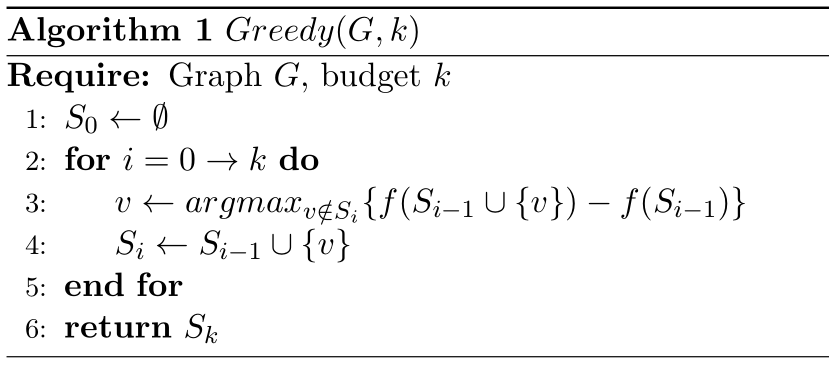
\includegraphics[width=4in]{images/greedy.png}
    \caption{贪心算法}\label{fig:greedy}
  \end{figure}

  但是显然这不是很好的做法,我们希望利用二分图的性质来改进算法时间复杂度.

  \begin{itemize}
  \item 之前的贪心算法在所有的节点之中搜索,这显然在二分图之中,是没有任何意义的,改变成只在节点集合A中进行搜索.
  \item 第二个就是传统的影响值计算十分复杂,效率低下,是采用了随机算法多次模拟传播过程,计算最终活跃节点数目,并取平均值.现在在二分图之中,我们可以采用更加快速的方法计算出精确的影响值来
  \item 第三个是一个启发式的改进思路,贪心算法的思想其实很简单,每一次循环都找到使得目标函数增长幅度最大的节点,然后加入到种子集合之中,但是我们每找一个节点都要把所有节点计算一遍,没有利用到之前的计算出来的信息,十分的慢。我的想法是基于一个假设,在一轮循环中,对目标函数贡献值大的节点但是没有被选为种子节点,在接下来的循环中极有可能被选为种子节点,所以我们可以优先计算这些节点的贡献值,这样的话,就可以减少很多不必要的计算。我的做法就是在找第一个节点的过程中使用一个优先队列来记录每一个节点对于目标函数的贡献,然后之后的每一次循环按照节点的贡献从大到小重新计算,然后到优先队列之中更新节点的贡献值。如果碰到某一个节点在一轮之中已经被计算过的话,那么这个节点就是我们想要的节点,它能使得目标函数的增长最大化,然后加入到种子节点之中。
  \end{itemize}

  图\ref{fig:new_greedy}为不加入启发式信息的改进算法。


  \begin{figure}[H]
    \centering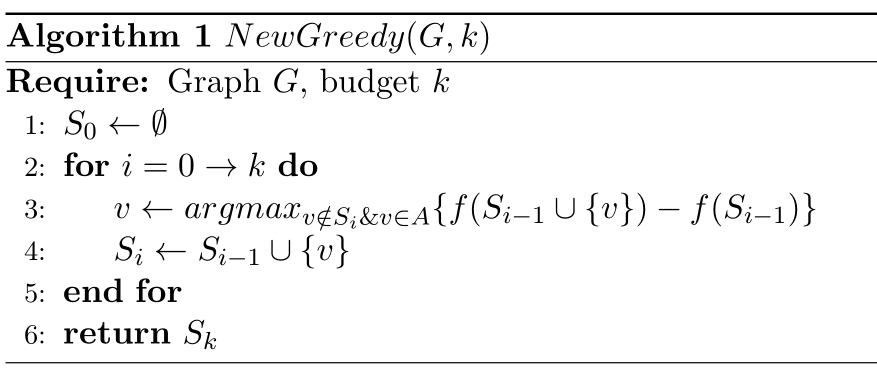
\includegraphics[width=4in]{images/new_greedy.png}
    \caption{不加入启发式信息的改进算法}\label{fig:new_greedy}
  \end{figure}


  算法中$f(S)$的计算变得更加快速,我们遍历集合B中的节点,计算集合A中所有节点对集合B中当前节点的影响力之和,(如果集合A中存在了三条到当前节点的边,权值分别是a,b,c,最终这个节点变成激活状态的可能性是$1-(1-a) (1-b) (1-c))$最后将集合B中所有节点受到的影响力加和得到了准确的结果.

  图\ref{fig:greedypp}为针对上面的算法加入启发式信息后的算法伪代码。

  \begin{figure}[H]
    \centering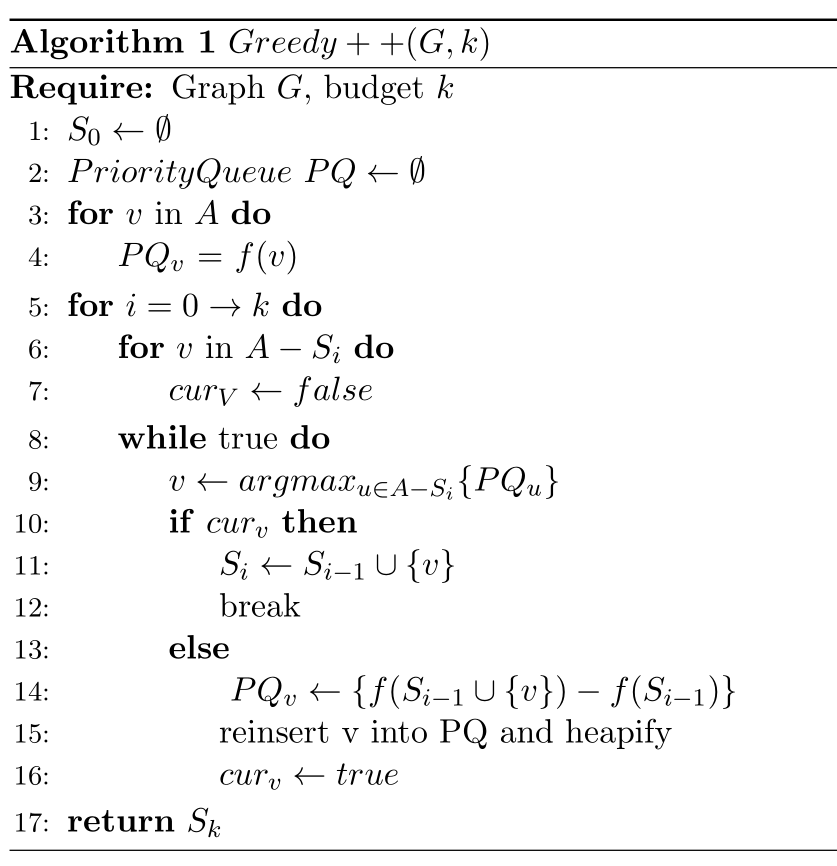
\includegraphics[width=4in]{images/greedypp.png}
    \caption{不加入启发式信息的改进算法}\label{fig:greedypp}
  \end{figure}

  \section{时间复杂度分析}

  假设输入的二分图包含n个节点,m条边,其中集合A中节点数目是a,集合B中节点数目是b.

  Greedy算法要循环k次,每一次需要遍历所有节点,计算每一个节点的影响贡献值,计算一个集合的影响值需要运行r遍ic模型,将求得的影响值取均值以减小误差,运行一次的时间复杂度是m,综上时间复杂度是$O(k\times n\times r\times m)$.

  NewGreedy同样需要运行k次,与Greedy所不同的是节点的选取只在集合A中,还有影响值的计算变的简单了,只需要计算一次,时间复杂度是k*b,所以总的时间复杂度是$O(k\times a\times k\times b)$.

  Greedy++的时间复杂度上界也是$O(k\times a\times k\times b)$,但是实际情况下,算法相比Newgreedy算法会很快停止.

  \section{实验部分}

  github 地址https://github.com/qioqio/IMP.git

  首先我们采用随机的方法生成了一个二分图,左边有30个节点,右边有30*50/20个节点,整个图之中,一共有30*50条边,并且边之中可能会有重复的边存在。第二个图是左边有300个节点,右边有300*500/20个节点,整个图之中,一共有300*500条边,并且边之中可能会有重复的边存在.然后将我们的算法应用到这个数据集合上,得到的效果非常不错,我们的算法比另外的一个启发式算法在二分图上表现的要好上不少。
  小图结果

  \section{未来的想法}

  如果我们继续挖掘这个问题的话,我们就会发现我们将youtube网站的用户分成两部分有合理性,但是集合A节点之间的相互影响也就是频道和频道之间的关系并不是完全不相关,频道的拥有者还是一个个的人,他们也在集合B之中,他们也会有自己收藏的一些频道,所以这些频道对于他自己的频道还是有影响的.如果考虑集合A节点之间的相互影响那么情况就会复杂一些.

  接下来,我们打算研究一些其他的社交网站的特性.比如说qq群.我们希望将qq群抽象成一个虚拟节点,这个节点和每一个成员节点之间有双向的边,边上的权值随机赋予(因为我们没有别的办法来衡量)(0.5 0.1 0.01)(具体如何赋值,我们可以参考其他的文献),接下来研究应该如何设计出算法.

  微信朋友圈里面的用户关系和知乎用户之间的关系和ic模型描述的拥有惊人的一致性,我们也希望可以爬取一些数据,进行一些算法设计.

\end{document}
